\documentclass[margin=2mm]{standalone}
\usepackage{tikz}
\usepackage{amsmath,amssymb,mathtools}
\begin{document}
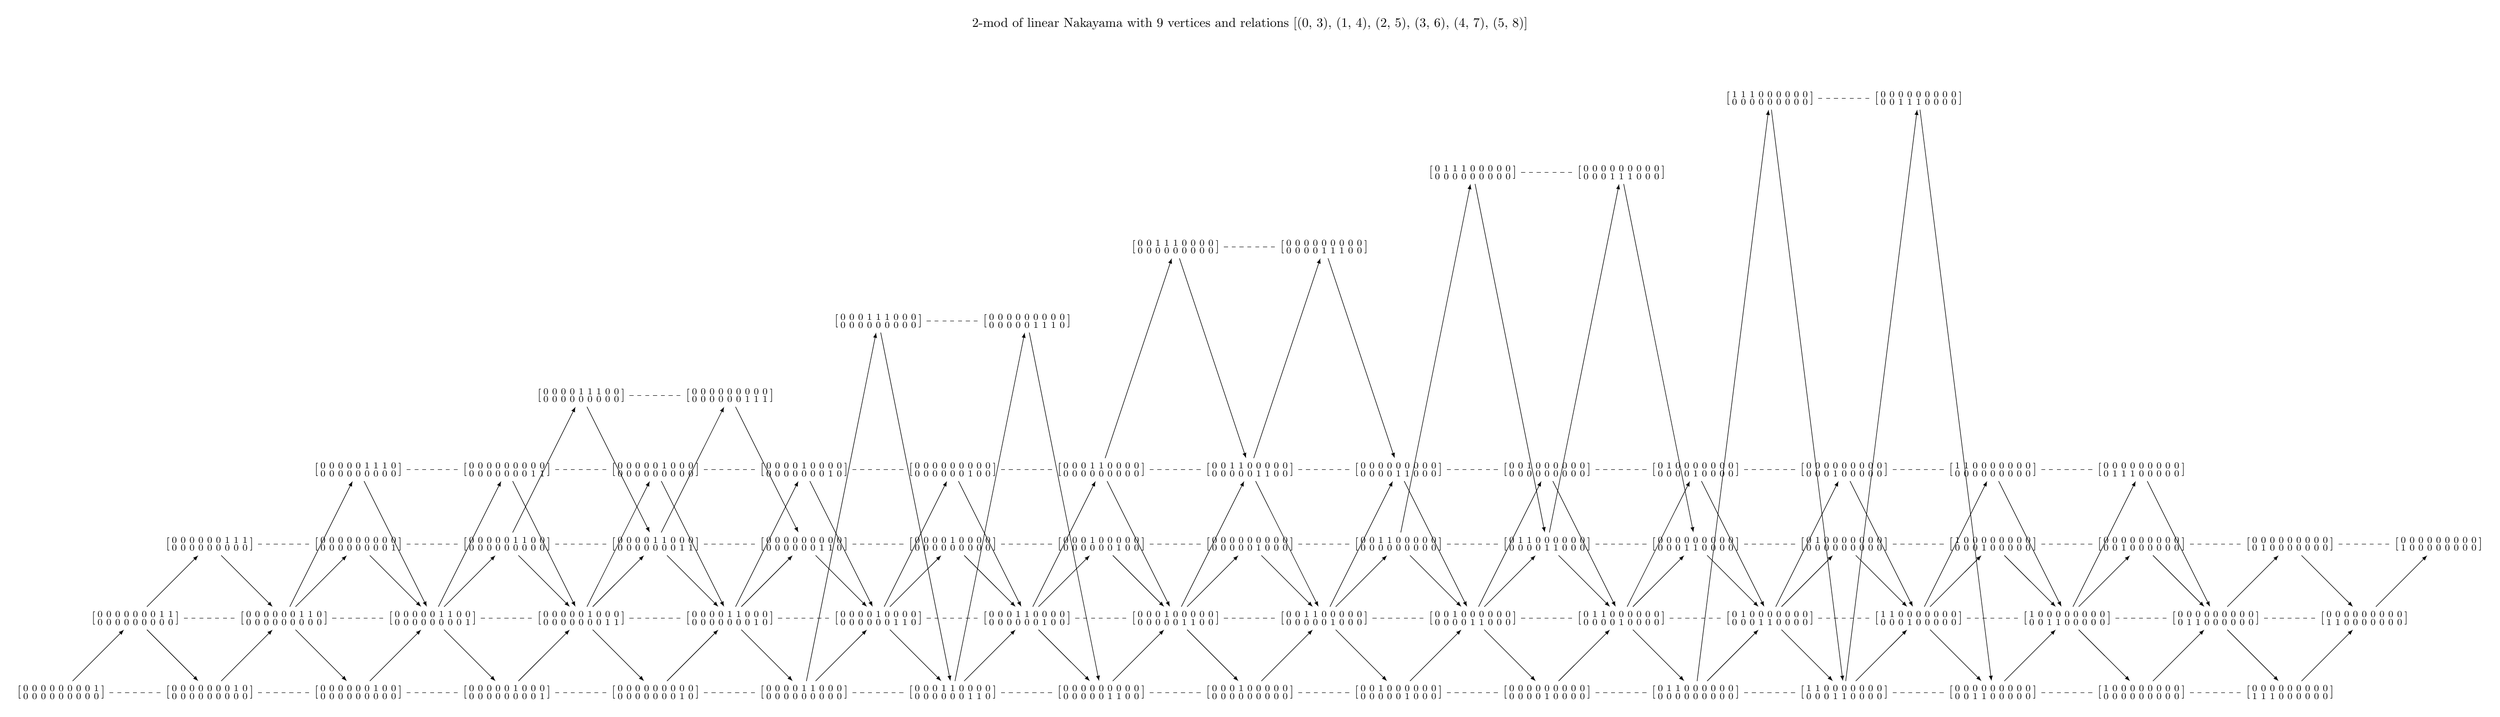
\begin{tikzpicture}[xscale=2,yscale=2]
\node at (16.0,9) [] {$2$-mod of linear Nakayama with 9 vertices and relations [(0, 3), (1, 4), (2, 5), (3, 6), (4, 7), (5, 8)]};
\node (t-0P0) at (23,8) [scale=1] {$\begin{bsmallmatrix}
 1 & 1 & 1 & 0 & 0 & 0 & 0 & 0 & 0\\
 0 & 0 & 0 & 0 & 0 & 0 & 0 & 0 & 0\\
\end{bsmallmatrix}$};
\node (t-1P0) at (25,8) [scale=1] {$\begin{bsmallmatrix}
 0 & 0 & 0 & 0 & 0 & 0 & 0 & 0 & 0\\
 0 & 0 & 1 & 1 & 1 & 0 & 0 & 0 & 0\\
\end{bsmallmatrix}$};
\node (t-0P1) at (19,7) [scale=1] {$\begin{bsmallmatrix}
 0 & 1 & 1 & 1 & 0 & 0 & 0 & 0 & 0\\
 0 & 0 & 0 & 0 & 0 & 0 & 0 & 0 & 0\\
\end{bsmallmatrix}$};
\node (t-1P1) at (21,7) [scale=1] {$\begin{bsmallmatrix}
 0 & 0 & 0 & 0 & 0 & 0 & 0 & 0 & 0\\
 0 & 0 & 0 & 1 & 1 & 1 & 0 & 0 & 0\\
\end{bsmallmatrix}$};
\node (t-0P2) at (15,6) [scale=1] {$\begin{bsmallmatrix}
 0 & 0 & 1 & 1 & 1 & 0 & 0 & 0 & 0\\
 0 & 0 & 0 & 0 & 0 & 0 & 0 & 0 & 0\\
\end{bsmallmatrix}$};
\node (t-1P2) at (17,6) [scale=1] {$\begin{bsmallmatrix}
 0 & 0 & 0 & 0 & 0 & 0 & 0 & 0 & 0\\
 0 & 0 & 0 & 0 & 1 & 1 & 1 & 0 & 0\\
\end{bsmallmatrix}$};
\node (t-0P3) at (11,5) [scale=1] {$\begin{bsmallmatrix}
 0 & 0 & 0 & 1 & 1 & 1 & 0 & 0 & 0\\
 0 & 0 & 0 & 0 & 0 & 0 & 0 & 0 & 0\\
\end{bsmallmatrix}$};
\node (t-1P3) at (13,5) [scale=1] {$\begin{bsmallmatrix}
 0 & 0 & 0 & 0 & 0 & 0 & 0 & 0 & 0\\
 0 & 0 & 0 & 0 & 0 & 1 & 1 & 1 & 0\\
\end{bsmallmatrix}$};
\node (t-0P4) at (7,4) [scale=1] {$\begin{bsmallmatrix}
 0 & 0 & 0 & 0 & 1 & 1 & 1 & 0 & 0\\
 0 & 0 & 0 & 0 & 0 & 0 & 0 & 0 & 0\\
\end{bsmallmatrix}$};
\node (t-1P4) at (9,4) [scale=1] {$\begin{bsmallmatrix}
 0 & 0 & 0 & 0 & 0 & 0 & 0 & 0 & 0\\
 0 & 0 & 0 & 0 & 0 & 0 & 1 & 1 & 1\\
\end{bsmallmatrix}$};
\node (t-0P5) at (4,3) [scale=1] {$\begin{bsmallmatrix}
 0 & 0 & 0 & 0 & 0 & 1 & 1 & 1 & 0\\
 0 & 0 & 0 & 0 & 0 & 0 & 0 & 0 & 0\\
\end{bsmallmatrix}$};
\node (t-1P5) at (6,3) [scale=1] {$\begin{bsmallmatrix}
 0 & 0 & 0 & 0 & 0 & 0 & 0 & 0 & 0\\
 0 & 0 & 0 & 0 & 0 & 0 & 0 & 1 & 1\\
\end{bsmallmatrix}$};
\node (t-2P5) at (8,3) [scale=1] {$\begin{bsmallmatrix}
 0 & 0 & 0 & 0 & 0 & 1 & 0 & 0 & 0\\
 0 & 0 & 0 & 0 & 0 & 0 & 0 & 0 & 0\\
\end{bsmallmatrix}$};
\node (t-3P5) at (10,3) [scale=1] {$\begin{bsmallmatrix}
 0 & 0 & 0 & 0 & 1 & 0 & 0 & 0 & 0\\
 0 & 0 & 0 & 0 & 0 & 0 & 0 & 1 & 0\\
\end{bsmallmatrix}$};
\node (t-4P5) at (12,3) [scale=1] {$\begin{bsmallmatrix}
 0 & 0 & 0 & 0 & 0 & 0 & 0 & 0 & 0\\
 0 & 0 & 0 & 0 & 0 & 0 & 1 & 0 & 0\\
\end{bsmallmatrix}$};
\node (t-5P5) at (14,3) [scale=1] {$\begin{bsmallmatrix}
 0 & 0 & 0 & 1 & 1 & 0 & 0 & 0 & 0\\
 0 & 0 & 0 & 0 & 0 & 0 & 0 & 0 & 0\\
\end{bsmallmatrix}$};
\node (t-6P5) at (16,3) [scale=1] {$\begin{bsmallmatrix}
 0 & 0 & 1 & 1 & 0 & 0 & 0 & 0 & 0\\
 0 & 0 & 0 & 0 & 0 & 1 & 1 & 0 & 0\\
\end{bsmallmatrix}$};
\node (t-7P5) at (18,3) [scale=1] {$\begin{bsmallmatrix}
 0 & 0 & 0 & 0 & 0 & 0 & 0 & 0 & 0\\
 0 & 0 & 0 & 0 & 1 & 1 & 0 & 0 & 0\\
\end{bsmallmatrix}$};
\node (t-8P5) at (20,3) [scale=1] {$\begin{bsmallmatrix}
 0 & 0 & 1 & 0 & 0 & 0 & 0 & 0 & 0\\
 0 & 0 & 0 & 0 & 0 & 0 & 0 & 0 & 0\\
\end{bsmallmatrix}$};
\node (t-9P5) at (22,3) [scale=1] {$\begin{bsmallmatrix}
 0 & 1 & 0 & 0 & 0 & 0 & 0 & 0 & 0\\
 0 & 0 & 0 & 0 & 1 & 0 & 0 & 0 & 0\\
\end{bsmallmatrix}$};
\node (t-10P5) at (24,3) [scale=1] {$\begin{bsmallmatrix}
 0 & 0 & 0 & 0 & 0 & 0 & 0 & 0 & 0\\
 0 & 0 & 0 & 1 & 0 & 0 & 0 & 0 & 0\\
\end{bsmallmatrix}$};
\node (t-11P5) at (26,3) [scale=1] {$\begin{bsmallmatrix}
 1 & 1 & 0 & 0 & 0 & 0 & 0 & 0 & 0\\
 0 & 0 & 0 & 0 & 0 & 0 & 0 & 0 & 0\\
\end{bsmallmatrix}$};
\node (t-12P5) at (28,3) [scale=1] {$\begin{bsmallmatrix}
 0 & 0 & 0 & 0 & 0 & 0 & 0 & 0 & 0\\
 0 & 1 & 1 & 1 & 0 & 0 & 0 & 0 & 0\\
\end{bsmallmatrix}$};
\node (t-0P6) at (2,2) [scale=1] {$\begin{bsmallmatrix}
 0 & 0 & 0 & 0 & 0 & 0 & 1 & 1 & 1\\
 0 & 0 & 0 & 0 & 0 & 0 & 0 & 0 & 0\\
\end{bsmallmatrix}$};
\node (t-1P6) at (4,2) [scale=1] {$\begin{bsmallmatrix}
 0 & 0 & 0 & 0 & 0 & 0 & 0 & 0 & 0\\
 0 & 0 & 0 & 0 & 0 & 0 & 0 & 0 & 1\\
\end{bsmallmatrix}$};
\node (t-2P6) at (6,2) [scale=1] {$\begin{bsmallmatrix}
 0 & 0 & 0 & 0 & 0 & 1 & 1 & 0 & 0\\
 0 & 0 & 0 & 0 & 0 & 0 & 0 & 0 & 0\\
\end{bsmallmatrix}$};
\node (t-3P6) at (8,2) [scale=1] {$\begin{bsmallmatrix}
 0 & 0 & 0 & 0 & 1 & 1 & 0 & 0 & 0\\
 0 & 0 & 0 & 0 & 0 & 0 & 0 & 1 & 1\\
\end{bsmallmatrix}$};
\node (t-4P6) at (10,2) [scale=1] {$\begin{bsmallmatrix}
 0 & 0 & 0 & 0 & 0 & 0 & 0 & 0 & 0\\
 0 & 0 & 0 & 0 & 0 & 0 & 1 & 1 & 0\\
\end{bsmallmatrix}$};
\node (t-5P6) at (12,2) [scale=1] {$\begin{bsmallmatrix}
 0 & 0 & 0 & 0 & 1 & 0 & 0 & 0 & 0\\
 0 & 0 & 0 & 0 & 0 & 0 & 0 & 0 & 0\\
\end{bsmallmatrix}$};
\node (t-6P6) at (14,2) [scale=1] {$\begin{bsmallmatrix}
 0 & 0 & 0 & 1 & 0 & 0 & 0 & 0 & 0\\
 0 & 0 & 0 & 0 & 0 & 0 & 1 & 0 & 0\\
\end{bsmallmatrix}$};
\node (t-7P6) at (16,2) [scale=1] {$\begin{bsmallmatrix}
 0 & 0 & 0 & 0 & 0 & 0 & 0 & 0 & 0\\
 0 & 0 & 0 & 0 & 0 & 1 & 0 & 0 & 0\\
\end{bsmallmatrix}$};
\node (t-8P6) at (18,2) [scale=1] {$\begin{bsmallmatrix}
 0 & 0 & 1 & 1 & 0 & 0 & 0 & 0 & 0\\
 0 & 0 & 0 & 0 & 0 & 0 & 0 & 0 & 0\\
\end{bsmallmatrix}$};
\node (t-9P6) at (20,2) [scale=1] {$\begin{bsmallmatrix}
 0 & 1 & 1 & 0 & 0 & 0 & 0 & 0 & 0\\
 0 & 0 & 0 & 0 & 1 & 1 & 0 & 0 & 0\\
\end{bsmallmatrix}$};
\node (t-10P6) at (22,2) [scale=1] {$\begin{bsmallmatrix}
 0 & 0 & 0 & 0 & 0 & 0 & 0 & 0 & 0\\
 0 & 0 & 0 & 1 & 1 & 0 & 0 & 0 & 0\\
\end{bsmallmatrix}$};
\node (t-11P6) at (24,2) [scale=1] {$\begin{bsmallmatrix}
 0 & 1 & 0 & 0 & 0 & 0 & 0 & 0 & 0\\
 0 & 0 & 0 & 0 & 0 & 0 & 0 & 0 & 0\\
\end{bsmallmatrix}$};
\node (t-12P6) at (26,2) [scale=1] {$\begin{bsmallmatrix}
 1 & 0 & 0 & 0 & 0 & 0 & 0 & 0 & 0\\
 0 & 0 & 0 & 1 & 0 & 0 & 0 & 0 & 0\\
\end{bsmallmatrix}$};
\node (t-13P6) at (28,2) [scale=1] {$\begin{bsmallmatrix}
 0 & 0 & 0 & 0 & 0 & 0 & 0 & 0 & 0\\
 0 & 0 & 1 & 0 & 0 & 0 & 0 & 0 & 0\\
\end{bsmallmatrix}$};
\node (t-14P6) at (30,2) [scale=1] {$\begin{bsmallmatrix}
 0 & 0 & 0 & 0 & 0 & 0 & 0 & 0 & 0\\
 0 & 1 & 0 & 0 & 0 & 0 & 0 & 0 & 0\\
\end{bsmallmatrix}$};
\node (t-15P6) at (32,2) [scale=1] {$\begin{bsmallmatrix}
 0 & 0 & 0 & 0 & 0 & 0 & 0 & 0 & 0\\
 1 & 0 & 0 & 0 & 0 & 0 & 0 & 0 & 0\\
\end{bsmallmatrix}$};
\node (t-0P7) at (1,1) [scale=1] {$\begin{bsmallmatrix}
 0 & 0 & 0 & 0 & 0 & 0 & 0 & 1 & 1\\
 0 & 0 & 0 & 0 & 0 & 0 & 0 & 0 & 0\\
\end{bsmallmatrix}$};
\node (t-1P7) at (3,1) [scale=1] {$\begin{bsmallmatrix}
 0 & 0 & 0 & 0 & 0 & 0 & 1 & 1 & 0\\
 0 & 0 & 0 & 0 & 0 & 0 & 0 & 0 & 0\\
\end{bsmallmatrix}$};
\node (t-2P7) at (5,1) [scale=1] {$\begin{bsmallmatrix}
 0 & 0 & 0 & 0 & 0 & 1 & 1 & 0 & 0\\
 0 & 0 & 0 & 0 & 0 & 0 & 0 & 0 & 1\\
\end{bsmallmatrix}$};
\node (t-3P7) at (7,1) [scale=1] {$\begin{bsmallmatrix}
 0 & 0 & 0 & 0 & 0 & 1 & 0 & 0 & 0\\
 0 & 0 & 0 & 0 & 0 & 0 & 0 & 1 & 1\\
\end{bsmallmatrix}$};
\node (t-4P7) at (9,1) [scale=1] {$\begin{bsmallmatrix}
 0 & 0 & 0 & 0 & 1 & 1 & 0 & 0 & 0\\
 0 & 0 & 0 & 0 & 0 & 0 & 0 & 1 & 0\\
\end{bsmallmatrix}$};
\node (t-5P7) at (11,1) [scale=1] {$\begin{bsmallmatrix}
 0 & 0 & 0 & 0 & 1 & 0 & 0 & 0 & 0\\
 0 & 0 & 0 & 0 & 0 & 0 & 1 & 1 & 0\\
\end{bsmallmatrix}$};
\node (t-6P7) at (13,1) [scale=1] {$\begin{bsmallmatrix}
 0 & 0 & 0 & 1 & 1 & 0 & 0 & 0 & 0\\
 0 & 0 & 0 & 0 & 0 & 0 & 1 & 0 & 0\\
\end{bsmallmatrix}$};
\node (t-7P7) at (15,1) [scale=1] {$\begin{bsmallmatrix}
 0 & 0 & 0 & 1 & 0 & 0 & 0 & 0 & 0\\
 0 & 0 & 0 & 0 & 0 & 1 & 1 & 0 & 0\\
\end{bsmallmatrix}$};
\node (t-8P7) at (17,1) [scale=1] {$\begin{bsmallmatrix}
 0 & 0 & 1 & 1 & 0 & 0 & 0 & 0 & 0\\
 0 & 0 & 0 & 0 & 0 & 1 & 0 & 0 & 0\\
\end{bsmallmatrix}$};
\node (t-9P7) at (19,1) [scale=1] {$\begin{bsmallmatrix}
 0 & 0 & 1 & 0 & 0 & 0 & 0 & 0 & 0\\
 0 & 0 & 0 & 0 & 1 & 1 & 0 & 0 & 0\\
\end{bsmallmatrix}$};
\node (t-10P7) at (21,1) [scale=1] {$\begin{bsmallmatrix}
 0 & 1 & 1 & 0 & 0 & 0 & 0 & 0 & 0\\
 0 & 0 & 0 & 0 & 1 & 0 & 0 & 0 & 0\\
\end{bsmallmatrix}$};
\node (t-11P7) at (23,1) [scale=1] {$\begin{bsmallmatrix}
 0 & 1 & 0 & 0 & 0 & 0 & 0 & 0 & 0\\
 0 & 0 & 0 & 1 & 1 & 0 & 0 & 0 & 0\\
\end{bsmallmatrix}$};
\node (t-12P7) at (25,1) [scale=1] {$\begin{bsmallmatrix}
 1 & 1 & 0 & 0 & 0 & 0 & 0 & 0 & 0\\
 0 & 0 & 0 & 1 & 0 & 0 & 0 & 0 & 0\\
\end{bsmallmatrix}$};
\node (t-13P7) at (27,1) [scale=1] {$\begin{bsmallmatrix}
 1 & 0 & 0 & 0 & 0 & 0 & 0 & 0 & 0\\
 0 & 0 & 1 & 1 & 0 & 0 & 0 & 0 & 0\\
\end{bsmallmatrix}$};
\node (t-14P7) at (29,1) [scale=1] {$\begin{bsmallmatrix}
 0 & 0 & 0 & 0 & 0 & 0 & 0 & 0 & 0\\
 0 & 1 & 1 & 0 & 0 & 0 & 0 & 0 & 0\\
\end{bsmallmatrix}$};
\node (t-15P7) at (31,1) [scale=1] {$\begin{bsmallmatrix}
 0 & 0 & 0 & 0 & 0 & 0 & 0 & 0 & 0\\
 1 & 1 & 0 & 0 & 0 & 0 & 0 & 0 & 0\\
\end{bsmallmatrix}$};
\node (t-0P8) at (0,0) [scale=1] {$\begin{bsmallmatrix}
 0 & 0 & 0 & 0 & 0 & 0 & 0 & 0 & 1\\
 0 & 0 & 0 & 0 & 0 & 0 & 0 & 0 & 0\\
\end{bsmallmatrix}$};
\node (t-1P8) at (2,0) [scale=1] {$\begin{bsmallmatrix}
 0 & 0 & 0 & 0 & 0 & 0 & 0 & 1 & 0\\
 0 & 0 & 0 & 0 & 0 & 0 & 0 & 0 & 0\\
\end{bsmallmatrix}$};
\node (t-2P8) at (4,0) [scale=1] {$\begin{bsmallmatrix}
 0 & 0 & 0 & 0 & 0 & 0 & 1 & 0 & 0\\
 0 & 0 & 0 & 0 & 0 & 0 & 0 & 0 & 0\\
\end{bsmallmatrix}$};
\node (t-3P8) at (6,0) [scale=1] {$\begin{bsmallmatrix}
 0 & 0 & 0 & 0 & 0 & 1 & 0 & 0 & 0\\
 0 & 0 & 0 & 0 & 0 & 0 & 0 & 0 & 1\\
\end{bsmallmatrix}$};
\node (t-4P8) at (8,0) [scale=1] {$\begin{bsmallmatrix}
 0 & 0 & 0 & 0 & 0 & 0 & 0 & 0 & 0\\
 0 & 0 & 0 & 0 & 0 & 0 & 0 & 1 & 0\\
\end{bsmallmatrix}$};
\node (t-5P8) at (10,0) [scale=1] {$\begin{bsmallmatrix}
 0 & 0 & 0 & 0 & 1 & 1 & 0 & 0 & 0\\
 0 & 0 & 0 & 0 & 0 & 0 & 0 & 0 & 0\\
\end{bsmallmatrix}$};
\node (t-6P8) at (12,0) [scale=1] {$\begin{bsmallmatrix}
 0 & 0 & 0 & 1 & 1 & 0 & 0 & 0 & 0\\
 0 & 0 & 0 & 0 & 0 & 0 & 1 & 1 & 0\\
\end{bsmallmatrix}$};
\node (t-7P8) at (14,0) [scale=1] {$\begin{bsmallmatrix}
 0 & 0 & 0 & 0 & 0 & 0 & 0 & 0 & 0\\
 0 & 0 & 0 & 0 & 0 & 1 & 1 & 0 & 0\\
\end{bsmallmatrix}$};
\node (t-8P8) at (16,0) [scale=1] {$\begin{bsmallmatrix}
 0 & 0 & 0 & 1 & 0 & 0 & 0 & 0 & 0\\
 0 & 0 & 0 & 0 & 0 & 0 & 0 & 0 & 0\\
\end{bsmallmatrix}$};
\node (t-9P8) at (18,0) [scale=1] {$\begin{bsmallmatrix}
 0 & 0 & 1 & 0 & 0 & 0 & 0 & 0 & 0\\
 0 & 0 & 0 & 0 & 0 & 1 & 0 & 0 & 0\\
\end{bsmallmatrix}$};
\node (t-10P8) at (20,0) [scale=1] {$\begin{bsmallmatrix}
 0 & 0 & 0 & 0 & 0 & 0 & 0 & 0 & 0\\
 0 & 0 & 0 & 0 & 1 & 0 & 0 & 0 & 0\\
\end{bsmallmatrix}$};
\node (t-11P8) at (22,0) [scale=1] {$\begin{bsmallmatrix}
 0 & 1 & 1 & 0 & 0 & 0 & 0 & 0 & 0\\
 0 & 0 & 0 & 0 & 0 & 0 & 0 & 0 & 0\\
\end{bsmallmatrix}$};
\node (t-12P8) at (24,0) [scale=1] {$\begin{bsmallmatrix}
 1 & 1 & 0 & 0 & 0 & 0 & 0 & 0 & 0\\
 0 & 0 & 0 & 1 & 1 & 0 & 0 & 0 & 0\\
\end{bsmallmatrix}$};
\node (t-13P8) at (26,0) [scale=1] {$\begin{bsmallmatrix}
 0 & 0 & 0 & 0 & 0 & 0 & 0 & 0 & 0\\
 0 & 0 & 1 & 1 & 0 & 0 & 0 & 0 & 0\\
\end{bsmallmatrix}$};
\node (t-14P8) at (28,0) [scale=1] {$\begin{bsmallmatrix}
 1 & 0 & 0 & 0 & 0 & 0 & 0 & 0 & 0\\
 0 & 0 & 0 & 0 & 0 & 0 & 0 & 0 & 0\\
\end{bsmallmatrix}$};
\node (t-15P8) at (30,0) [scale=1] {$\begin{bsmallmatrix}
 0 & 0 & 0 & 0 & 0 & 0 & 0 & 0 & 0\\
 1 & 1 & 1 & 0 & 0 & 0 & 0 & 0 & 0\\
\end{bsmallmatrix}$};
\draw[-latex] (t-0P0) -- (t-12P8);
\draw[-latex] (t-1P0) -- (t-13P8);
\draw[-latex] (t-0P1) -- (t-9P6);
\draw[-latex] (t-1P1) -- (t-10P6);
\draw[-latex] (t-0P2) -- (t-6P5);
\draw[-latex] (t-1P2) -- (t-7P5);
\draw[-latex] (t-0P3) -- (t-6P8);
\draw[-latex] (t-1P3) -- (t-7P8);
\draw[-latex] (t-0P4) -- (t-3P6);
\draw[-latex] (t-1P4) -- (t-4P6);
\draw[-latex] (t-0P5) -- (t-2P7);
\draw[-latex] (t-1P5) -- (t-3P7);
\draw[-latex] (t-2P5) -- (t-4P7);
\draw[-latex] (t-3P5) -- (t-5P7);
\draw[-latex] (t-4P5) -- (t-6P7);
\draw[-latex] (t-5P5) -- (t-0P2);
\draw[-latex] (t-5P5) -- (t-7P7);
\draw[-latex] (t-6P5) -- (t-1P2);
\draw[-latex] (t-6P5) -- (t-8P7);
\draw[-latex] (t-7P5) -- (t-9P7);
\draw[-latex] (t-8P5) -- (t-10P7);
\draw[-latex] (t-9P5) -- (t-11P7);
\draw[-latex] (t-10P5) -- (t-12P7);
\draw[-latex] (t-11P5) -- (t-13P7);
\draw[-latex] (t-12P5) -- (t-14P7);
\draw[-latex] (t-0P6) -- (t-1P7);
\draw[-latex] (t-1P6) -- (t-2P7);
\draw[-latex] (t-2P6) -- (t-0P4);
\draw[-latex] (t-2P6) -- (t-3P7);
\draw[-latex] (t-3P6) -- (t-4P7);
\draw[-latex] (t-3P6) -- (t-1P4);
\draw[-latex] (t-4P6) -- (t-5P7);
\draw[-latex] (t-5P6) -- (t-6P7);
\draw[-latex] (t-6P6) -- (t-7P7);
\draw[-latex] (t-7P6) -- (t-8P7);
\draw[-latex] (t-8P6) -- (t-0P1);
\draw[-latex] (t-8P6) -- (t-9P7);
\draw[-latex] (t-9P6) -- (t-10P7);
\draw[-latex] (t-9P6) -- (t-1P1);
\draw[-latex] (t-10P6) -- (t-11P7);
\draw[-latex] (t-11P6) -- (t-12P7);
\draw[-latex] (t-12P6) -- (t-13P7);
\draw[-latex] (t-13P6) -- (t-14P7);
\draw[-latex] (t-14P6) -- (t-15P7);
\draw[-latex] (t-0P7) -- (t-0P6);
\draw[-latex] (t-0P7) -- (t-1P8);
\draw[-latex] (t-1P7) -- (t-0P5);
\draw[-latex] (t-1P7) -- (t-1P6);
\draw[-latex] (t-1P7) -- (t-2P8);
\draw[-latex] (t-2P7) -- (t-1P5);
\draw[-latex] (t-2P7) -- (t-2P6);
\draw[-latex] (t-2P7) -- (t-3P8);
\draw[-latex] (t-3P7) -- (t-2P5);
\draw[-latex] (t-3P7) -- (t-3P6);
\draw[-latex] (t-3P7) -- (t-4P8);
\draw[-latex] (t-4P7) -- (t-3P5);
\draw[-latex] (t-4P7) -- (t-4P6);
\draw[-latex] (t-4P7) -- (t-5P8);
\draw[-latex] (t-5P7) -- (t-4P5);
\draw[-latex] (t-5P7) -- (t-5P6);
\draw[-latex] (t-5P7) -- (t-6P8);
\draw[-latex] (t-6P7) -- (t-5P5);
\draw[-latex] (t-6P7) -- (t-6P6);
\draw[-latex] (t-6P7) -- (t-7P8);
\draw[-latex] (t-7P7) -- (t-6P5);
\draw[-latex] (t-7P7) -- (t-7P6);
\draw[-latex] (t-7P7) -- (t-8P8);
\draw[-latex] (t-8P7) -- (t-7P5);
\draw[-latex] (t-8P7) -- (t-8P6);
\draw[-latex] (t-8P7) -- (t-9P8);
\draw[-latex] (t-9P7) -- (t-8P5);
\draw[-latex] (t-9P7) -- (t-9P6);
\draw[-latex] (t-9P7) -- (t-10P8);
\draw[-latex] (t-10P7) -- (t-9P5);
\draw[-latex] (t-10P7) -- (t-10P6);
\draw[-latex] (t-10P7) -- (t-11P8);
\draw[-latex] (t-11P7) -- (t-10P5);
\draw[-latex] (t-11P7) -- (t-11P6);
\draw[-latex] (t-11P7) -- (t-12P8);
\draw[-latex] (t-12P7) -- (t-11P5);
\draw[-latex] (t-12P7) -- (t-12P6);
\draw[-latex] (t-12P7) -- (t-13P8);
\draw[-latex] (t-13P7) -- (t-12P5);
\draw[-latex] (t-13P7) -- (t-13P6);
\draw[-latex] (t-13P7) -- (t-14P8);
\draw[-latex] (t-14P7) -- (t-14P6);
\draw[-latex] (t-14P7) -- (t-15P8);
\draw[-latex] (t-15P7) -- (t-15P6);
\draw[-latex] (t-0P8) -- (t-0P7);
\draw[-latex] (t-1P8) -- (t-1P7);
\draw[-latex] (t-2P8) -- (t-2P7);
\draw[-latex] (t-3P8) -- (t-3P7);
\draw[-latex] (t-4P8) -- (t-4P7);
\draw[-latex] (t-5P8) -- (t-0P3);
\draw[-latex] (t-5P8) -- (t-5P7);
\draw[-latex] (t-6P8) -- (t-6P7);
\draw[-latex] (t-6P8) -- (t-1P3);
\draw[-latex] (t-7P8) -- (t-7P7);
\draw[-latex] (t-8P8) -- (t-8P7);
\draw[-latex] (t-9P8) -- (t-9P7);
\draw[-latex] (t-10P8) -- (t-10P7);
\draw[-latex] (t-11P8) -- (t-0P0);
\draw[-latex] (t-11P8) -- (t-11P7);
\draw[-latex] (t-12P8) -- (t-12P7);
\draw[-latex] (t-12P8) -- (t-1P0);
\draw[-latex] (t-13P8) -- (t-13P7);
\draw[-latex] (t-14P8) -- (t-14P7);
\draw[-latex] (t-15P8) -- (t-15P7);
\draw[dashed] (t-0P0)--(t-1P0);
\draw[dashed] (t-0P1)--(t-1P1);
\draw[dashed] (t-0P2)--(t-1P2);
\draw[dashed] (t-0P3)--(t-1P3);
\draw[dashed] (t-0P4)--(t-1P4);
\draw[dashed] (t-0P5)--(t-1P5);
\draw[dashed] (t-1P5)--(t-2P5);
\draw[dashed] (t-2P5)--(t-3P5);
\draw[dashed] (t-3P5)--(t-4P5);
\draw[dashed] (t-4P5)--(t-5P5);
\draw[dashed] (t-5P5)--(t-6P5);
\draw[dashed] (t-6P5)--(t-7P5);
\draw[dashed] (t-7P5)--(t-8P5);
\draw[dashed] (t-8P5)--(t-9P5);
\draw[dashed] (t-9P5)--(t-10P5);
\draw[dashed] (t-10P5)--(t-11P5);
\draw[dashed] (t-11P5)--(t-12P5);
\draw[dashed] (t-0P6)--(t-1P6);
\draw[dashed] (t-1P6)--(t-2P6);
\draw[dashed] (t-2P6)--(t-3P6);
\draw[dashed] (t-3P6)--(t-4P6);
\draw[dashed] (t-4P6)--(t-5P6);
\draw[dashed] (t-5P6)--(t-6P6);
\draw[dashed] (t-6P6)--(t-7P6);
\draw[dashed] (t-7P6)--(t-8P6);
\draw[dashed] (t-8P6)--(t-9P6);
\draw[dashed] (t-9P6)--(t-10P6);
\draw[dashed] (t-10P6)--(t-11P6);
\draw[dashed] (t-11P6)--(t-12P6);
\draw[dashed] (t-12P6)--(t-13P6);
\draw[dashed] (t-13P6)--(t-14P6);
\draw[dashed] (t-14P6)--(t-15P6);
\draw[dashed] (t-0P7)--(t-1P7);
\draw[dashed] (t-1P7)--(t-2P7);
\draw[dashed] (t-2P7)--(t-3P7);
\draw[dashed] (t-3P7)--(t-4P7);
\draw[dashed] (t-4P7)--(t-5P7);
\draw[dashed] (t-5P7)--(t-6P7);
\draw[dashed] (t-6P7)--(t-7P7);
\draw[dashed] (t-7P7)--(t-8P7);
\draw[dashed] (t-8P7)--(t-9P7);
\draw[dashed] (t-9P7)--(t-10P7);
\draw[dashed] (t-10P7)--(t-11P7);
\draw[dashed] (t-11P7)--(t-12P7);
\draw[dashed] (t-12P7)--(t-13P7);
\draw[dashed] (t-13P7)--(t-14P7);
\draw[dashed] (t-14P7)--(t-15P7);
\draw[dashed] (t-0P8)--(t-1P8);
\draw[dashed] (t-1P8)--(t-2P8);
\draw[dashed] (t-2P8)--(t-3P8);
\draw[dashed] (t-3P8)--(t-4P8);
\draw[dashed] (t-4P8)--(t-5P8);
\draw[dashed] (t-5P8)--(t-6P8);
\draw[dashed] (t-6P8)--(t-7P8);
\draw[dashed] (t-7P8)--(t-8P8);
\draw[dashed] (t-8P8)--(t-9P8);
\draw[dashed] (t-9P8)--(t-10P8);
\draw[dashed] (t-10P8)--(t-11P8);
\draw[dashed] (t-11P8)--(t-12P8);
\draw[dashed] (t-12P8)--(t-13P8);
\draw[dashed] (t-13P8)--(t-14P8);
\draw[dashed] (t-14P8)--(t-15P8);
\end{tikzpicture}\end{document}